% !TEX root = ../ac_paper.tex

\section{Language Modeling} \label{sec:lm}

In this section, we discuss a model for the ``language" of balanced presentations. Each presentation with two relators is a sequence made of six letters, also known as ``tokens" in the nomenclature of Natural Language Processing, i.e. $x$, $y$, $x^{-1}$, and $y^{-1}$, and two ``stop tokens" --- one that separates two relators of a presentation, and another that marks the end of a presentation. Given this vocabulary $V$ of six tokens, we can ask what is the probability $p(t_1, \cdots, t_N)$ for $t_i \in V$ of the occurence of a specific presentation in the space of all balanced presentations. Using the chain rule of probability theory, 
\[
p(t_1 \cdots t_{N}) = \prod\limits_{i=1}^{N} p (t_{i} \mid t_{1} \cdots t_{i-1}) 
\]

Here $p (t_{N} \mid t_{1} \cdots t_{N-1})$, often called the $N$-gram probability distribution, is the probability of a token $t_N$ following a sequence of tokens $t_{1} \cdots t_{N-1}$. To model the language of balanced presentations, we can alternatively estimate the $N$-gram probability distributions for all $N$. 

Over the last few years, Transformer models have shown great success in modeling human-understandable languages to the extent that these models can write text almost indistinguishable from human-written texts. Specifically, the architecture used for modeling language is the auto-regressive ``decoder-only" Transformer, which we review in detail in \autoref{sec:transformer_review}. In \autoref{sec:transformer_datasets}, we discuss the method with which we generate the dataset required for training the model. Finally, in \autoref{sec:transformer_results}, we provide details of some insights we learn from this process. 

\subsection{Transformers: a review\label{sec:transformer_review}}

Here, we give a short review of the architecture of a decoder-only transformer. For more detailed descriptions, see \cite{vaswani2023attention, elhage2021mathematical, douglas2023large}. 

Given an input sequence $t_1, t_2, \cdots, t_{N}$, a decoder-only transformer predicts the probability distribution $p(t \mid t_1, t_2, \cdots, t_{N})$ over the set $V$ of tokens of size $n_{\text{vocab}}$. The probability is computed by applying the softmax function to the logits $T(t)$, which are estimated by applying the following sequence of operations.
\footnote{The softmax function, $\softmax: \mathbb{R}^n \to (0, 1)^{n}$, is defined as $\softmax(x)_i = e^{x_i} / \sum\limits_{j=1}^n e^{x_j}$.}

First, assign to each token in the vocabulary a distinct label in the range $1, 2, \cdots, n_{\text{vocab}}$; re-writing the original sequence as a sequence of integers, which we also label as $t_i$. Next, write the sequence in terms of ``one-hot encoded vectors", i.e. a matrix $t  \in \R^{N \times n_{\text{vocab}}}$ such that 
\[
t_{ij} = \delta_{i t_i}
\]
and embed the sequence in a $\dm$-dimensional vector space, \fixme{I think this should be $(W_P \otimes 1 + 1 \otimes W_E) t$}
\[
x_0 = (W_P \otimes W_E) t
\]
Here, $W_P \in \R^{\dm \times N}$ and $W_E \in \R^{\dm \times n_{\text{vocab}} }$ are positional and token embedding matrices, which are learned by gradient descent. 
\footnote{Note that $t$ and all $x_j$ are two-dimensional tensors, so it is appropriate to apply tensors of linear transformations to them. Often in a transformer architecture, these operations are of the form $\mathbb{1} \otimes \cdots$; in these cases, we drop the identity transformation and simply write the operation as $\cdots$. For example, $\mathbb{1} \otimes W_U$, $\mathbb{1} \otimes W^m_I$, $\mathbb{1} \otimes W^m_O$, etc. are all often simply written as $W_U$, $W^m_I$, $W^m_O$ respectively. It is clear from the dimensionality of these matrices that they are tensored with identity transformations.}
An $L$-layer transformer alternates between applying a ``multi-head attention layer" ($\sum\limits_{h \in H} h$) and an ``MLP-layer" ($m$) $L$ times. For $i=0, \cdots, L-1$,
\[
\begin{aligned}
x_{2i+1} &= x_{2i} + \sum_{h \in H} h(\LN(x_{2i})), \\
x_{2i + 2} &= x_{2i + 1} + m(\LN(x_{2i + 1})).
\end{aligned}
\]
Each $x_j$ is an element of $\mathbb{R^{N \times \dm}}$, with the interpretation that its $i$-th row is the embedding of the sequence $t_1, \cdots, t_i$ in the embedding space $\mathbb{R}^{\dm}$ as learned by the preceeding $j+1$ operations. Finally, one applies an ``unembedding layer", $W_U \in \mathbb{R}^{n_{\text{vocab}} \times \dm}$, to convert the output of the final layer to an $n_{\text{vocab}}$-dimensional vector of logits that estimate the sought-after probability distribution.
\[
\begin{aligned}
T(t) &= W_U x_{2L-1} \\
p(t) &=\softmax (T(t))
\end{aligned}
\]

The functions $\LN$, $m$ and $h$ are defined as follows. $\LN$ is the "Layer-Norm" operation intended to normalize the input of each layer to make the optimization process more feasible,
\[
LN(x) = \left(\mathbb{1} \otimes \text{diag}(\gamma) \right) \frac{(x-\overline{x})}{\sqrt{\text{var}(x)}} + \mathbb{1} \otimes \beta
\]
Here, $\gamma, \beta \in \mathbb{R}^{\dm}$ are learnable parameters. $\overline{x}$ and $\text{var}(x)$ are mean and variance of each row of $x$.

The MLP-layer $m$ is a non-linear operation, 
\[
m(x) =W^m_O \ \text{max}(W_I^m x, 0)
\]
with learnable parameters $W^m_I \in \mathbb{R}^{d_{\text{MLP}} \times \dm}$, $W^m_O \in \mathbb{R}^{\dm \times d_{\text{MLP}}}$. It is standard to set $d_{\text{MLP}} = 4 \dm$.

Finally, the multi-headed attention-layer $\sum_{h \in H} h$ is a sum of $n_{\text{heads}}$ ``attention-head" operations $h$, 
\[
h(x) = (A^h(x) \otimes W^h_O W^h_V) x
\]
where $W^h_V \in \R^{d_{\text{head}} \times \dm}$, 
$W^h_O \in \R^{\dm \times d_{\text{head}}}$ 
are matrices of learnable parameters. 
$d_{\text{head}}$ is the ``attention-head dimension" that satisfies $d_{\text{head}} \times n_{\text{head}} = d_{\text{model}}$. 
The attention matrix $A^h$ is computed with the help of learnable matrices 
$W^h_Q, W^h_K \in \R^{d_{\text{head}} \times \dm}$,
\[
A^h(x) = \softmax^\star \left(\frac{x^T (W^h_Q)^T W^h_K x}{\sqrt{d_{\text{head}}}}\right)
\] 
The attention-head is an $N \times N$ matrix. The element $A^h(x)_{ij}$ 
is interpreted as the ``attention" paid to the token 
$t_j$ in estimating 
$p(t_{i+1} \mid t_1, \cdots, t_i)$. $\softmax^\star$
is a variant of the $\softmax$ function suitable for auto-regressive tasks: it sets the upper triangular part of its input to zeros before applying the 
$\softmax$ operation. 
That is, future tokens --- $t_k$ for $k > i$, play no role in the prediction of $p(t_{i+1} \mid t_1, \cdots, t_i)$.

We train the transformer model by minimizing the cross-entropy loss between the estimated and the true probability distributions of $p(t_{i+1} | t_1, \cdots, t_{i})$ for all $i$. The parallelism offered by the processing of all tokens in a sequence at once is extremely useful for efficient training of a model for language modeling task.

Before we discuss the dataset we used to train our model, we present an important remark. In practice, the embedding matrix $W_E$ and the unembedding matrix $W_U$ are often ``tied" together, i.e. $W_E = W_U^T$ \cite{press2017using, inan2017tying}.
The rows of $W_E = W_U^T$ are interpreted as the embeddings of words/sentences, to which one may apply the usual operations of a vector space \cite{Bengio:2003, mikolov-etal-2013-linguistic}. 
For example, the cosine of the angle between two embedding vectors, also known as ``cosine similarity", is often used to measure the similarity between two texts. 
Two semantically similar texts have higher cosine similarity between them, while semantically different texts correspond to (almost) orthogonal vectors in the embedding space.


\subsection{Training and Evaluation Datasets\label{sec:transformer_datasets}}

We now discuss the training and validation datasets used to train and evaluate our Transformer model. As our main interest in this paper has been in the presentations of the Miller-Schupp series, we generated a dataset of balanced presentations that are AC-equivalent to the Miller-Schupp presentations. Specifically, we apply sequences of AC moves to the 1190 presentations with $n,\ \text{length}(w) \leq 7$ discussed in \autoref{sec:AC}, creating a dataset of about 1.8 million presentations. Approximately 1 million of these presentations are AC-equivalent to the GS-hard presentations of section 3, while the remaining are related to the GS-easy presentations. 
Only a small amount (roughly 15 percent) of the original Miller-Schupp presentations were part of this dataset.

The dataset is tokenized using six tokens: two stop tokens and one token each for the two generators and their inverses. The tokenized dataset had about $2.17 \times 10^8$ tokens. As our hope is to get insights into properties that distinguish GS-easy and GS-hard presentations, we perform an exploratory data analysis of the two subsets of data associated to these presentations. We plot the percentage of appearance of each token for these subsets in \autoref{fig:tokens_hist}. 
Note that the ratio of frequency of $y^{\pm 1}$ to the frequency of $x^{\pm 1}$ is higher in the GS-hard dataset. This is likely because the GS-hard presentations have larger $n$, and larger $n$ corresponds to a higher number of occurence of $y^{\pm 1}$ in the Miller-Schupp presentation. Interestingly, this effect remains in the dataset even when after applying thousands of AC moves to the original presentations.

We paid special attention to ensure that our dataset contains presentations of a wide range of total lengths so as not to bias our model towards learning trends specific to any fixed length. To this end, we devised an algorithm (\autoref{alg:apply_ac_moves} in \autoref{app:algorithm}) that creates an almost uniform distribution over the total lengths of the presentations. (See \autoref{fig:gpt_data}.) We also remark that we set aside $10\%$ of our entire data as a validation dataset.

\begin{figure}
	\centering
	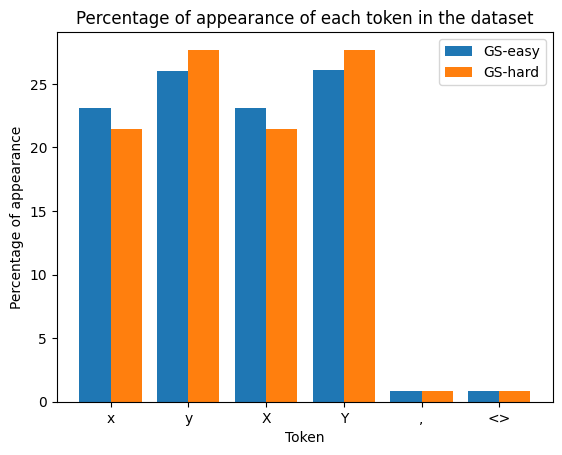
\includegraphics[scale=0.6]{fig/tokens_hist.png}
	\caption{Percentage of appearance of each token in the two subsets of the training dataset that are equivalent to GS-easy and GS-hard presentations. To be clear, we computed the percentages separately for each subset of the training data, i.e. the heights of all blue (and orange) bars adds separately to 100.}
	\label{fig:tokens_hist}
\end{figure}


\begin{figure}
	\centering
	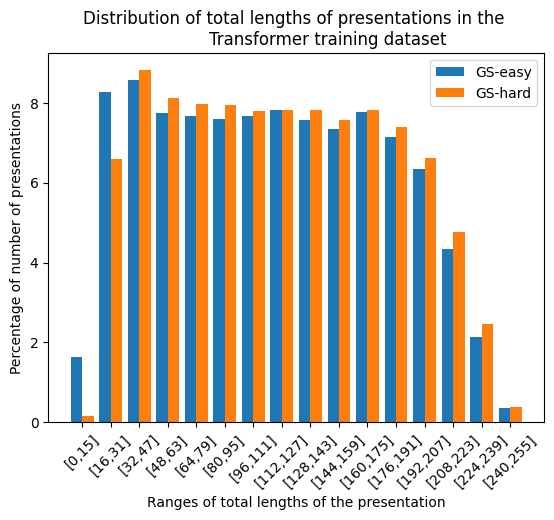
\includegraphics[scale=0.6]{fig/gpt_data_length_distribution.png}
	\caption{Percentage of presentations in various ranges of total lengths. Percentages were computed independently for the two subsets of the dataset, corresponding to presentations that are AC-equivalent to GS-easy and GS-hard presentations. We used \autoref{alg:apply_ac_moves} from \autoref{app:algorithm} to ensure the almost-uniform distribution depicted here.}
	\label{fig:gpt_data}
\end{figure}




\subsection{Results\label{sec:transformer_results}}
Finally, we discuss the results of our experiments. We trained a Transformer model with hyperparameters given in  \autoref{app:hyperparameters}. A randomly initialized model with initialization scheme given in \cite{Radford2019LanguageMA} has a validation loss of $~1.8$, while the trained model could achieve a validation loss of $0.7337$.
\footnote{We tuned the hyperparameters a little but it is quite likely that one can achieve a better performing model with more hyperparameter tuning. Similarly, more training data will necessarily help with the performance}
We used the untrained (randomly initialized) and the trained model to get embeddings of all presentations of the Miller-Schupp series discussed in \autoref{sec:AC}. We used t-SNE to project these embedding vectors to a plane \cite{JMLR:v9:vandermaaten08a}. These plots are shown in a $7 \times 2$ grid in \autoref{fig:tsne_embeddings}.

Each row of \autoref{fig:tsne_embeddings} corresponds to a fixed value of $n$. The left column depicts t-SNE projections of embeddings obtained by an untrained model, while the right column shows the embeddings of a trained Transformer model. We note that the GS-easy and GS-hard presentations seem to cluster much more in the plots in the right column. This indicates that a trained Transformer model is able to distinguish between GS-easy and GS-hard presentations to a good extent, albeit not perfectly. 

Note that the training dataset of Transformer contained no information about the easy of solvability of a presentation. It also did not contain many presentations of the Miller-Schupp series itself. Instead, it was made of presentations of varying lengths that are AC-equivalent to the Miller-Schupp series presentations. This indicates that a). there could likely be an invariant at the level of the ``language`` of the balanced presentations that distinguishes easy vs hard presentations, and b). this invariant survives application of thousands of AC moves which we used to generate the 
training examples in our dataset. 

 Note that t-SNE dependence on a distance measure: it learns to map the vectors that are closer together in the higher-dimensional space with respect to this distance measure, close together in the plane. We used cosine simiarity between embedding vectors as the distance measure for our plots. Note also that t-SNE admits a hyperparameter known as ``perplexity", and the projections learned by t-SNE depend on the hyperparameter \cite{wattenberg2016how}. Thus, in general, t-SNE plots must be interpreted with care. The plots shown in \autoref{fig:tsne_embeddings} were all made with the perplexity value of $30$, though, we have checked that the clustering of GS-easy and GS-hard presentations seems to exist at a broad range of perplexity values.




\begin{figure}
    \centering
    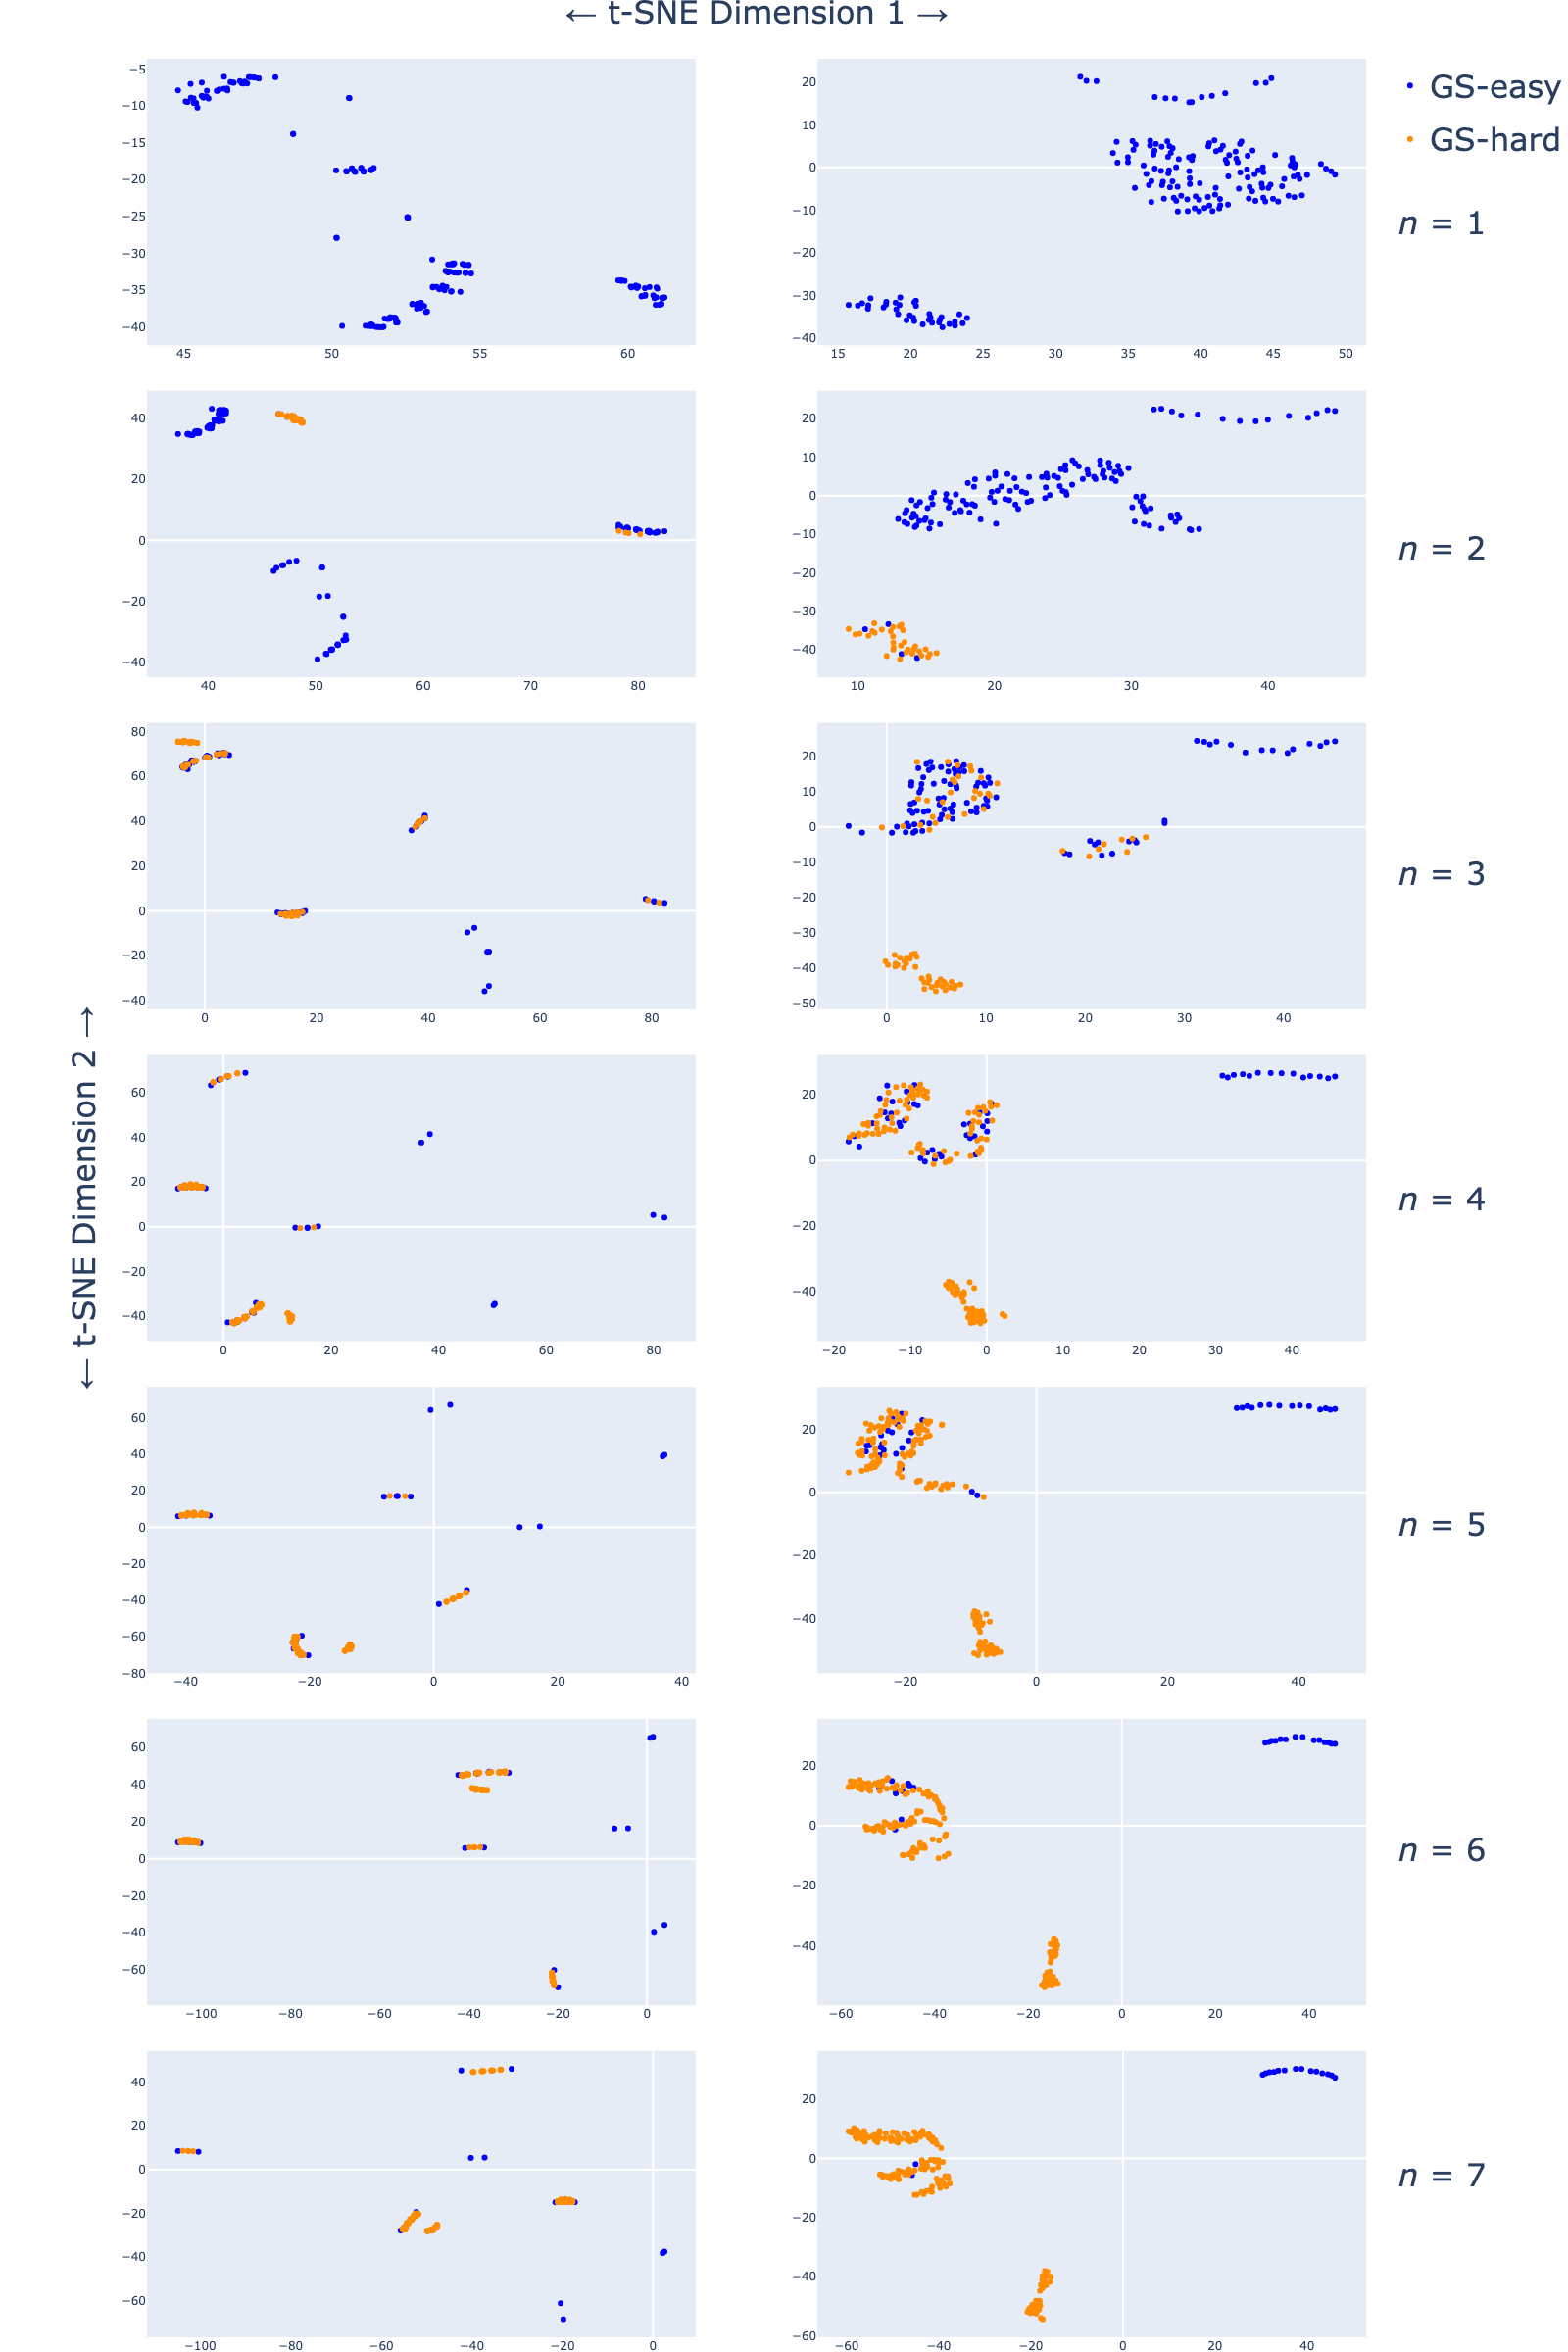
\includegraphics[scale=0.23]{fig/embeddings.png}
    \captionsetup{width=1.1\textwidth}
    \caption{t-SNE plots depicting embeddings of the Miller-Schupp presentations $MS(n, w)$. The left (right) column shows embeddings learned by an untrained (trained) transformer model. Each row corresponds to a value of $n$. Trained models cluster together GS-easy and GS-hard presentations indicating the possibility of a difference in the linguistic structure of the two sets of presentations.}
    \label{fig:tsne_embeddings}
\end{figure}
